% Created by tikzDevice version 0.7.0 on 2014-10-06 19:44:25
% !TEX encoding = UTF-8 Unicode
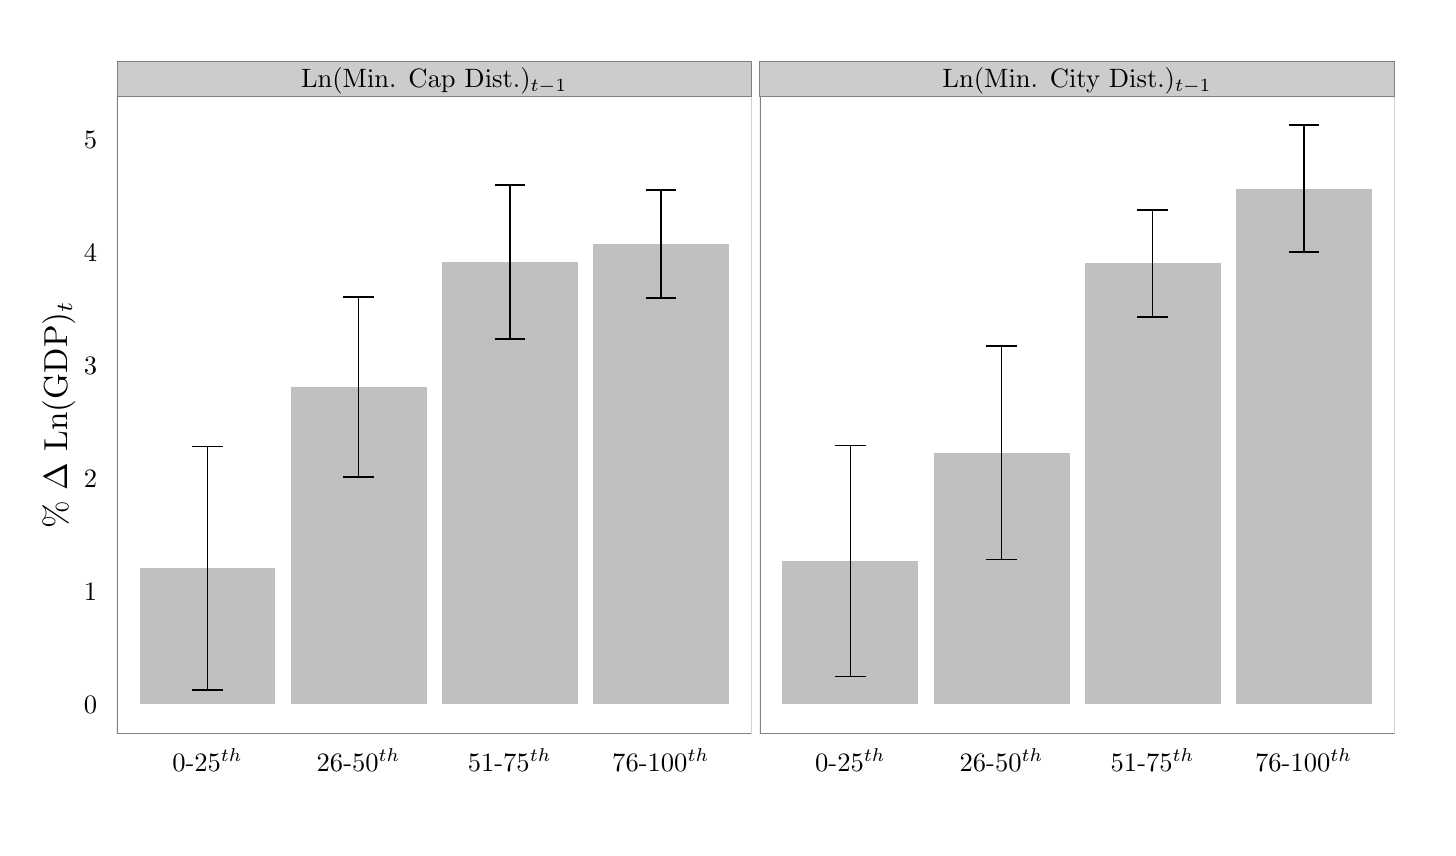
\begin{tikzpicture}[x=1pt,y=1pt]
\definecolor[named]{fillColor}{rgb}{1.00,1.00,1.00}
\path[use as bounding box,fill=fillColor,fill opacity=0.00] (0,0) rectangle (505.89,289.08);
\begin{scope}
\path[clip] (  0.00,  0.00) rectangle (505.89,289.08);
\definecolor[named]{drawColor}{rgb}{1.00,1.00,1.00}
\definecolor[named]{fillColor}{rgb}{1.00,1.00,1.00}

\path[draw=drawColor,line width= 0.6pt,line join=round,line cap=round,fill=fillColor] (  0.00,  0.00) rectangle (505.89,289.08);
\end{scope}
\begin{scope}
\path[clip] ( 32.22, 34.03) rectangle (261.53,264.40);
\definecolor[named]{fillColor}{rgb}{1.00,1.00,1.00}

\path[fill=fillColor] ( 32.22, 34.03) rectangle (261.53,264.40);
\definecolor[named]{fillColor}{rgb}{0.75,0.75,0.75}

\path[fill=fillColor] ( 40.41, 44.51) rectangle ( 89.55, 93.75);

\path[fill=fillColor] ( 95.01, 44.51) rectangle (144.14,159.24);

\path[fill=fillColor] (149.60, 44.51) rectangle (198.74,204.41);

\path[fill=fillColor] (204.20, 44.51) rectangle (253.34,210.90);
\definecolor[named]{drawColor}{rgb}{0.00,0.00,0.00}

\path[draw=drawColor,line width= 0.6pt,line join=round] ( 59.52,137.78) --
	( 70.44,137.78);

\path[draw=drawColor,line width= 0.6pt,line join=round] ( 64.98,137.78) --
	( 64.98, 49.72);

\path[draw=drawColor,line width= 0.6pt,line join=round] ( 59.52, 49.72) --
	( 70.44, 49.72);

\path[draw=drawColor,line width= 0.6pt,line join=round] (114.12,191.72) --
	(125.04,191.72);

\path[draw=drawColor,line width= 0.6pt,line join=round] (119.58,191.72) --
	(119.58,126.77);

\path[draw=drawColor,line width= 0.6pt,line join=round] (114.12,126.77) --
	(125.04,126.77);

\path[draw=drawColor,line width= 0.6pt,line join=round] (168.71,232.19) --
	(179.63,232.19);

\path[draw=drawColor,line width= 0.6pt,line join=round] (174.17,232.19) --
	(174.17,176.63);

\path[draw=drawColor,line width= 0.6pt,line join=round] (168.71,176.63) --
	(179.63,176.63);

\path[draw=drawColor,line width= 0.6pt,line join=round] (223.31,230.44) --
	(234.23,230.44);

\path[draw=drawColor,line width= 0.6pt,line join=round] (228.77,230.44) --
	(228.77,191.36);

\path[draw=drawColor,line width= 0.6pt,line join=round] (223.31,191.36) --
	(234.23,191.36);
\definecolor[named]{drawColor}{rgb}{0.50,0.50,0.50}

\path[draw=drawColor,line width= 0.6pt,line join=round,line cap=round] ( 32.22, 34.03) rectangle (261.53,264.40);
\end{scope}
\begin{scope}
\path[clip] (264.54, 34.03) rectangle (493.85,264.40);
\definecolor[named]{fillColor}{rgb}{1.00,1.00,1.00}

\path[fill=fillColor] (264.54, 34.03) rectangle (493.85,264.40);
\definecolor[named]{fillColor}{rgb}{0.75,0.75,0.75}

\path[fill=fillColor] (272.73, 44.51) rectangle (321.87, 96.35);

\path[fill=fillColor] (327.33, 44.51) rectangle (376.46,135.46);

\path[fill=fillColor] (381.92, 44.51) rectangle (431.06,203.89);

\path[fill=fillColor] (436.52, 44.51) rectangle (485.66,230.96);
\definecolor[named]{drawColor}{rgb}{0.00,0.00,0.00}

\path[draw=drawColor,line width= 0.6pt,line join=round] (291.84,138.07) --
	(302.76,138.07);

\path[draw=drawColor,line width= 0.6pt,line join=round] (297.30,138.07) --
	(297.30, 54.63);

\path[draw=drawColor,line width= 0.6pt,line join=round] (291.84, 54.63) --
	(302.76, 54.63);

\path[draw=drawColor,line width= 0.6pt,line join=round] (346.43,174.04) --
	(357.35,174.04);

\path[draw=drawColor,line width= 0.6pt,line join=round] (351.89,174.04) --
	(351.89, 96.87);

\path[draw=drawColor,line width= 0.6pt,line join=round] (346.43, 96.87) --
	(357.35, 96.87);

\path[draw=drawColor,line width= 0.6pt,line join=round] (401.03,223.16) --
	(411.95,223.16);

\path[draw=drawColor,line width= 0.6pt,line join=round] (406.49,223.16) --
	(406.49,184.61);

\path[draw=drawColor,line width= 0.6pt,line join=round] (401.03,184.61) --
	(411.95,184.61);

\path[draw=drawColor,line width= 0.6pt,line join=round] (455.63,253.93) --
	(466.55,253.93);

\path[draw=drawColor,line width= 0.6pt,line join=round] (461.09,253.93) --
	(461.09,208.00);

\path[draw=drawColor,line width= 0.6pt,line join=round] (455.63,208.00) --
	(466.55,208.00);
\definecolor[named]{drawColor}{rgb}{0.50,0.50,0.50}

\path[draw=drawColor,line width= 0.6pt,line join=round,line cap=round] (264.54, 34.03) rectangle (493.85,264.40);
\end{scope}
\begin{scope}
\path[clip] (  0.00,  0.00) rectangle (505.89,289.08);
\definecolor[named]{drawColor}{rgb}{0.50,0.50,0.50}
\definecolor[named]{fillColor}{rgb}{0.80,0.80,0.80}

\path[draw=drawColor,line width= 0.2pt,line join=round,line cap=round,fill=fillColor] ( 32.22,264.40) rectangle (261.53,277.04);
\definecolor[named]{drawColor}{rgb}{0.00,0.00,0.00}

\node[text=drawColor,anchor=base,inner sep=0pt, outer sep=0pt, scale=  0.96] at (146.87,267.41) {Ln(Min. Cap Dist.)$_{t-1}$};
\end{scope}
\begin{scope}
\path[clip] (  0.00,  0.00) rectangle (505.89,289.08);
\definecolor[named]{drawColor}{rgb}{0.50,0.50,0.50}
\definecolor[named]{fillColor}{rgb}{0.80,0.80,0.80}

\path[draw=drawColor,line width= 0.2pt,line join=round,line cap=round,fill=fillColor] (264.54,264.40) rectangle (493.85,277.04);
\definecolor[named]{drawColor}{rgb}{0.00,0.00,0.00}

\node[text=drawColor,anchor=base,inner sep=0pt, outer sep=0pt, scale=  0.96] at (379.19,267.41) {Ln(Min. City Dist.)$_{t-1}$};
\end{scope}
\begin{scope}
\path[clip] (  0.00,  0.00) rectangle (505.89,289.08);
\definecolor[named]{drawColor}{rgb}{0.00,0.00,0.00}

\node[text=drawColor,anchor=base east,inner sep=0pt, outer sep=0pt, scale=  0.96] at ( 25.11, 41.20) {0};

\node[text=drawColor,anchor=base east,inner sep=0pt, outer sep=0pt, scale=  0.96] at ( 25.11, 82.02) {1};

\node[text=drawColor,anchor=base east,inner sep=0pt, outer sep=0pt, scale=  0.96] at ( 25.11,122.84) {2};

\node[text=drawColor,anchor=base east,inner sep=0pt, outer sep=0pt, scale=  0.96] at ( 25.11,163.67) {3};

\node[text=drawColor,anchor=base east,inner sep=0pt, outer sep=0pt, scale=  0.96] at ( 25.11,204.49) {4};

\node[text=drawColor,anchor=base east,inner sep=0pt, outer sep=0pt, scale=  0.96] at ( 25.11,245.31) {5};
\end{scope}
\begin{scope}
\path[clip] (  0.00,  0.00) rectangle (505.89,289.08);
\definecolor[named]{drawColor}{rgb}{0.00,0.00,0.00}

\node[text=drawColor,anchor=base,inner sep=0pt, outer sep=0pt, scale=  0.96] at ( 64.98, 20.31) {0-25$^{th}$};

\node[text=drawColor,anchor=base,inner sep=0pt, outer sep=0pt, scale=  0.96] at (119.58, 20.31) {26-50$^{th}$};

\node[text=drawColor,anchor=base,inner sep=0pt, outer sep=0pt, scale=  0.96] at (174.17, 20.31) {51-75$^{th}$};

\node[text=drawColor,anchor=base,inner sep=0pt, outer sep=0pt, scale=  0.96] at (228.77, 20.31) {76-100$^{th}$};
\end{scope}
\begin{scope}
\path[clip] (  0.00,  0.00) rectangle (505.89,289.08);
\definecolor[named]{drawColor}{rgb}{0.00,0.00,0.00}

\node[text=drawColor,anchor=base,inner sep=0pt, outer sep=0pt, scale=  0.96] at (297.30, 20.31) {0-25$^{th}$};

\node[text=drawColor,anchor=base,inner sep=0pt, outer sep=0pt, scale=  0.96] at (351.89, 20.31) {26-50$^{th}$};

\node[text=drawColor,anchor=base,inner sep=0pt, outer sep=0pt, scale=  0.96] at (406.49, 20.31) {51-75$^{th}$};

\node[text=drawColor,anchor=base,inner sep=0pt, outer sep=0pt, scale=  0.96] at (461.09, 20.31) {76-100$^{th}$};
\end{scope}
\begin{scope}
\path[clip] (  0.00,  0.00) rectangle (505.89,289.08);
\definecolor[named]{drawColor}{rgb}{0.00,0.00,0.00}

\node[text=drawColor,rotate= 90.00,anchor=base,inner sep=0pt, outer sep=0pt, scale=  1.20] at ( 14.29,149.22) {\% $\Delta$ Ln(GDP)$_{t}$};
\end{scope}
\end{tikzpicture}
